\documentclass{amsart}
\usepackage{graphicx}
\graphicspath{{./}}
\usepackage{hyperref}
\usepackage{csvsimple}
\usepackage{longtable}
\usepackage{epigraph}
\title{Ethnicity Effects on Moral Views about Beating Wife}
\author{Zulfikar Moinuddin Ahmed}
\date{\today}
\begin{document}
\maketitle

\section{Introduction}

In America there are various horrible rumours about all sorts of people having propensity to beat their wives.  We'll take a deeper look in actual measured data.

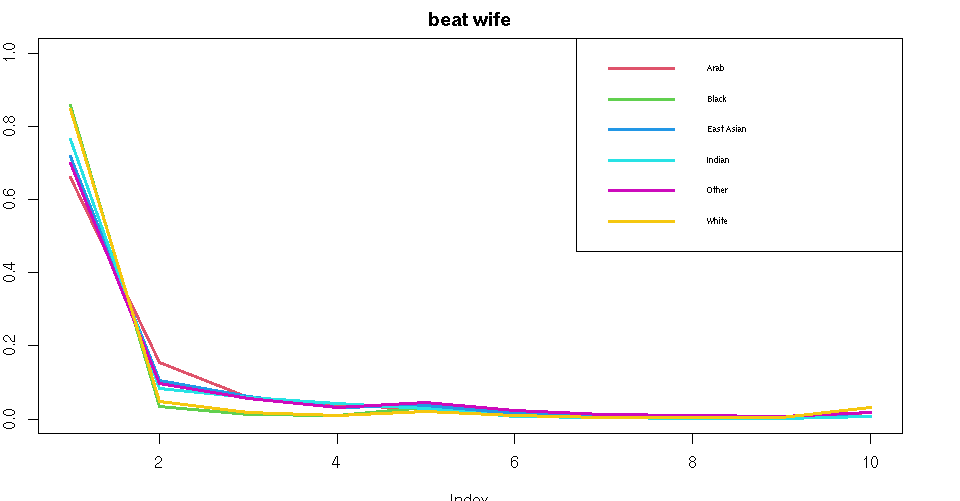
\includegraphics[scale=0.5]{ethbeatwife.jpeg}

% latex table generated in R 4.0.3 by xtable 1.8-4 package
% Mon May 10 02:40:44 2021
\begin{table}[ht]
\centering
\begin{tabular}{rlr}
  \hline
 & eth & explained \\ 
  \hline
1 & Arab & 3.16 \\ 
  2 & Black & 1.98 \\ 
  3 & East Asian & 0.46 \\ 
  4 & Indian & 0.11 \\ 
  5 & Other & 0.77 \\ 
  6 & White & 1.50 \\ 
   \hline
\end{tabular}
\end{table}

None of these effects are particularly strong.  Let's look at the percentages that are in 1-5 (don't find beating wife justifiable).
% latex table generated in R 4.0.3 by xtable 1.8-4 package
% Mon May 10 02:46:08 2021
\begin{table}[ht]
\centering
\begin{tabular}{rlr}
  \hline
 & eth & good \\ 
  \hline
1 & Arab & 94.16 \\ 
  2 & Black & 94.47 \\ 
  3 & East Asian & 95.39 \\ 
  4 & Indian & 97.69 \\ 
  5 & Other & 92.92 \\ 
  6 & White & 94.23 \\ 
   \hline
\end{tabular}
\end{table}

There is no significant difference at all between percentages of Arabs, Whites, Blacks in those who find wife beating unjustified.

\section{Conclusion}

Don't have prejudices against other people considering them 'wife beaters'.  This is highly offensive and wrong.

\end{document}